%!TEX root = ../thesis.tex
\begin{savequote}[75mm]
Nulla facilisi. In vel sem. Morbi id urna in diam dignissim feugiat. Proin molestie tortor eu velit. Aliquam erat volutpat. Nullam ultrices, diam tempus vulputate egestas, eros pede varius leo.
\qauthor{Quoteauthor Lastname}
\end{savequote}

%\chapter{\textsc{The internship project}}
\chapter{The internship project}

%\newthought{There's something to be said} for having a good opening line. Morbi commodo, ipsum sed pharetra gravida, orci  $x = 1/\alpha$ magna rhoncus neque, id pulvinar odio lorem non turpis \cite{Eigen1971, Knuth1968}. Nullam sit amet enim. Suspendisse id velit vitae ligula volutpat condimentum. Aliquam erat volutpat. Sed quis velit. Nulla facilisi. Nulla libero. Vivamus pharetra posuere sapien. Nam consectetuer. Sed aliquam, nunc eget euismod ullamcorper, lectus nunc ullamcorper orci, fermentum bibendum enim nibh eget ipsum. Donec porttitor ligula eu dolor. Maecenas vitae nulla consequat libero cursus venenatis. Nam magna enim, accumsan eu, blandit sed, blandit a, eros.
%$$\zeta = \frac{1039}{\pi}$$

% For an example of a full page figure, see Fig.~\ref{fig:myFullPageFigure}.

This chapter is all about the discussions and planification that has been made prior to the beginning of the internship.

It includes the results of the discussions with the tutor (Dr. Fabio Giust) and the creation of the piano di lavoro document che spiega in maniera più dettagliata questo capitolo

In here is also described how a resolution for the problem was first thought and how it was 

\section{The company's needs}
che cosa sta utilizzando athonet adesso per la gestione del lavoro e del tracking\\
come issue tracking system, gestore di wiki interno, ecc --> tanti tool scorrelati tra loro\\
perchè athonet ha la necessità di utilizzare tool differenti \\
(+ stabili, meglio documentati, miglior UI / UX etc.)

\section{Planning}
in base a cosa ho pianificato
come ho parlato con il tutor per fare capire i loro bisogni, lo scopo finale, e come arrivarci
step da fare\\
parlare poi di chi avrà bisogno del tool e con chi interagirò durante lo stage\\
fase preliminare di pianificazione insieme ad altre figure (aree diverse, managemeng, product ownership...)

\section{Approaching the problem}

	After the discussion with the tutor I have studied the arguments that we have talked about and formalized the requirements into some objectives

\section{The work plan}

	To formalize the previous discussions and create a followable roadmap, I have created a work plan document that contains a Gantt diagram and a table that describes the hours spent per task.
	
	This document, formally called "Piano di lavoro"
	
	This document tries to be an
	
	\section{Time suddivisione}
	
		\begin{figure}[H]
			\centering
			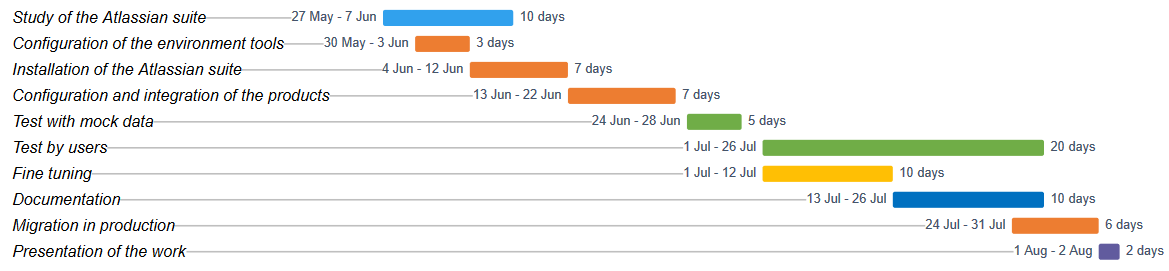
\includegraphics[width=1.1\textwidth]{resources/work_plan_gantt}\\
			\caption{Gantt diagram contained in the ``\textit{Piano di Lavoro}'' document}
		\end{figure}

		Spiegare che in questo documento viene quindi spiegato che è stato deciso di fare lo stage della durata di 10 settimane

	\section{Requirements}
	
		Definizione dei requisiti, messa in un piano di lavoro, mettere in appendice
	
